\documentclass[12pt, a4paper, titlepage, table]{article}
\usepackage{pdfpages}
\usepackage[utf8]{inputenc}
\usepackage[T1]{fontenc}
\usepackage{titlesec}
\usepackage[french]{babel}
\usepackage{caption}
\usepackage{float}
\usepackage{graphicx}
\usepackage[inner=2cm, outer=2cm, top=2cm, bottom=2cm]{geometry}
\usepackage[T1]{fontenc}
\usepackage{times}
\usepackage{xr} 
\usepackage{multirow}
\usepackage{amsmath}
\usepackage{array}
\usepackage{booktabs}
\usepackage{tabularx}
\usepackage{ragged2e}
\usepackage{adjustbox}

\begin{document}
	\label{document}
	\title{Etude de l'insertion professionnelle des diplômés de l'université (DUT, Licence Pro, MASTER LMD et Master ENS)}
	\author{Sébastien Mertès}
	\date{\today}
	\maketitle
	\renewcommand{\thesection}{\arabic{section}.}
	\renewcommand{\thesubsection}{\thesection\arabic{subsection}}
	\renewcommand{\tablename}{Tableau}
	\renewcommand{\abstractname}{Résumé}
	\captionsetup[table]{font={small}}
	\setlength{\parindent}{0pt}
	\captionsetup{labelfont=bf, font=small}
	\tableofcontents
	\newcolumntype{C}{>{\RaggedRight\arraybackslash}X}
	\newpage
	
\section{Introduction}
	
\section{Présentation des données}
	Nous avons 3 jeux de données représentant respectivement les informations concernant l'évaluation de l'insertion professionnelle sur le marché du travail des diplômés universitaires en DUT, Licence Professionnelle, Master LMD (Licence-Master-Doctorat) et Master ENS (Enseignement) de toutes les disciplines. 
	
	Ces données ont été collectées 18 mois et 30 mois après l'obtention du diplôme des sessions  2013 à 2019. Ainsi l'enquête a commencé en décembre 2015, pour s'achever en décembre 2021.
	
	Les données collectées regroupent, par niveau de diplôme, les disciplines, le taux d'insertion, le salaire brut et net estimé, le pourcentage des types de contrat professionnel (CDI, CDD, intérimaire etc...) ainsi que les secteurs d'activité, les professions et le type d'entreprises.
	
	Les tableaux 1 à 5 décrivent les différentes variables utilisées pour cette étude et le taux en pourcentage de valeurs manquantes de chaque modalité pour les les différentes catégories.
	
	Le Tableaux 1, présente la liste des diplômes universitaires pour les DUT, Licence Professionnelle et MASTERS.
	Les MASTERS sont distingués par le MASTER LMD et le MASTER ENS. 
	
	Les disciplines sont indiquées aussi bien individuellement (Informatique, histoire, droit, psychologie etc..), que par des ensembles de disciplines (Formations juridiques, économiques et de gestion, Sciences humaines et sociales etc...). L'ensemble de toutes les disciplines par niveau de diplôme est aussi indiqué (Ensemble MASTERS LMD, Ensemble des départements d'IUT etc...).   
	
	
	
\newpage

\begin{table}[H]
	\centering
	\begin{adjustbox}{max width=\textwidth}
		\begin{tabularx}{\linewidth}{|l|C|}
			\hline
			\multicolumn{1}{|c|}{\textbf{Diplôme}} & \multicolumn{1}{c|}{\textbf{Définition}} \\
			\hline
			DUT & Diplôme Universitaire de Technologie. Formation de 2 ans axée sur des compétences techniques et pratiques. \\
			\hline
			LICENCE PRO & Licence professionnelle. Programme de 1 an après un DUT ou une Licence, offrant une spécialisation professionnelle. \\
			\hline
			MASTER ENS & Master Enseignement. Diplôme permettant de devenir enseignant dans le système éducatif français. \\
			\hline
			MASTER LMD & Système européen d'enseignement supérieur avec niveaux de Licence, Master et Doctorat. \\
			\hline
		\end{tabularx}
	\end{adjustbox}
	\caption{Nom de la variable catégorielle et ses modalités concernant les diplômes universitaires}
	\label{tab:diplomes}
\end{table}

\begin{table}[H]
	\centering
	\begin{adjustbox}{max width=\textwidth}
	\begin{tabularx}{\linewidth}{|l|C|}
		\hline
		\multicolumn{1}{|c|}{\textbf{Discipline}} & \multicolumn{1}{c|}{\textbf{Ensemble}} \\
		\hline
		Autres sciences humaines et sociales & Ensemble Licence professionnelle \\
		\hline
		Autres formations juridiques, économiques et de gestion & Ensemble formations juridiques, économiques et de gestion \\
		\hline
		Sciences de la vie et de la terre & Ensemble des départements d'IUT \\
		\hline
		Psychologie & Ensemble sciences humaines et sociales \\
		\hline
		Information communication & Ensemble sciences, technologies et santé \\
		\hline
		Lettres, langues, arts & Autres sciences, technologies et santé \\
		\hline
		Sciences de l'ingénieur & Ensemble Masters LMD (hors Masters enseignement et hors Dauphine et Antilles-Guyane) \\
		\hline
		Histoire-géographie & Ensemble Masters LMD (hors Masters enseignement) \\
		\hline
		Droit & \\
		\hline
		Informatique & \\
		\hline
		Gestion & \\
		\hline
		Sciences fondamentales & \\
		\hline
		Économie & \\
		\hline
		Masters enseignement & \\
		\hline
	\end{tabularx}
	\end{adjustbox}
	\caption{Liste des disciplines et ensembles}
	\label{tab:disciplines}
\end{table}


\begin{table}[H]
	\centering
	\begin{tabularx}{\textwidth}{|X|c|}
		\hline
		\textbf{Contrat} & \textbf{\%} \\
		\hline
		Prof. libérale, indépendant, chef d’entreprise & 8.1 \\
		\hline
		Fonctionnaire & 8.1 \\
		\hline
		CDI & 8.1 \\
		\hline
		CDI de chantier ou CDI de mission & 8.8 \\
		\hline
		Contrat spécifique au doctorat & 10.5 \\
		\hline
		CDD & 8.1 \\
		\hline
		Vacataire & 8.1 \\
		\hline
		Intérimaire & 8.1 \\
		\hline
		Intermittent du spectacle & 8.1 \\
		\hline
		Contrat de professionnalisation & 8.1 \\
		\hline
		Emplois aidés (Contrat Initiative Emploi…) & 8.1 \\
		\hline
		Volontariat international & 8.1 \\
		\hline
	\end{tabularx}
	\caption{Pourcentage de valeurs manquantes des différents types de contrat}
	\label{tab:contrats_pourcentage}
\end{table}

\begin{table}[H]
	\centering
	\begin{tabularx}{\textwidth}{|X|c|}
		\hline
		\textbf{Entreprise} & \textbf{\%} \\
		\hline
		Vous-même & 11.0 \\
		\hline
		La fonction publique (d'etat, territoriale ou hospitalière) & 11.0 \\
		\hline
		Une entreprise privée & 11.0 \\
		\hline
		Une entreprise publique & 11.0 \\
		\hline
		Une association & 11.0 \\
		\hline
		Une personne exerçant une profession libérale ou un indépendant & 11.0 \\
		\hline
		Organisation internationale ou une institution de l'Union européenne & 11.5 \\
		\hline
		Société d'économie mixte & 11.4 \\
		\hline
		Un particulier & 11.0 \\
		\hline
	\end{tabularx}
	\caption{Pourcentage de valeurs manquantes par type d'entreprise}
	\label{tab:entreprise_pourcentage}
\end{table}


\begin{table}[H]
	\centering
	\begin{tabularx}{\textwidth}{|X|c|}
		\hline
		\textbf{Secteur} & \textbf{\%} \\
		\hline
		Agriculture, sylviculture et pêche & 7.1 \\
		\hline
		Industries (manufacturières, extractives et autres) & 7.1 \\
		\hline
		Construction & 7.1 \\
		\hline
		Activités immobilières & 7.4 \\
		\hline
		Commerce, transports, hébergement et restauration & 7.1 \\
		\hline
		Information et communication & 7.1 \\
		\hline
		Activités financières et d’assurance & 7.1 \\
		\hline
		Activités spécialisées, scientifiques et techniques & 7.1 \\
		\hline
		Activités de services administratifs et de soutien & 7.1 \\
		\hline
		Enseignement & 7.1 \\
		\hline
		Administration publique (hors enseignement) & 7.1 \\
		\hline
		Santé humaine et action sociale & 7.1 \\
		\hline
		Arts, spectacles et activités récréatives & 7.1 \\
		\hline
		Autres activités de service & 7.1 \\
		\hline
	\end{tabularx}
	\caption{Pourcentage de valeurs manquantes par secteur}
	\label{tab:secteurs_pourcentage}
\end{table}

\begin{table}[H]
	\centering
	\begin{tabularx}{\textwidth}{|X|c|}
		\hline
		\textbf{Profession} & \textbf{\%} \\
		\hline
		Agriculteur & 11.2 \\
		\hline
		Artisan, commerçant, chef d'entreprise & 11.1 \\
		\hline
		Profession libérale & 11.1 \\
		\hline
		Personnel de catégorie A de la fonction publique & 10.2 \\
		\hline
		Ingénieur, cadre, professions libérales, professions intellectuelles supérieures & 10.2 \\
		\hline
		Personnel de catégorie B de la fonction publique & 10.2 \\
		\hline
		Emploi de niveau intermédiaire : technicien, agent de maîtrise, etc. & 10.2 \\
		\hline
		Personnel de catégorie C de la fonction publique & 10.2 \\
		\hline
		Manœuvre, ouvrier & 10.2 \\
		\hline
		Employé de bureau, de commerce, personnel de service & 5.3 \\
		\hline
	\end{tabularx}
	\caption{Pourcentage de valeurs manquantes par profession}
	\label{tab:professions_pourcentage}
\end{table}


\section{Les types de contrats après l'obtention du diplôme}

	\subsection{Répartion des contrats à 18 et 30 mois après l'obtention du diplôme}
		\begin{figure}[H]
			\centering
			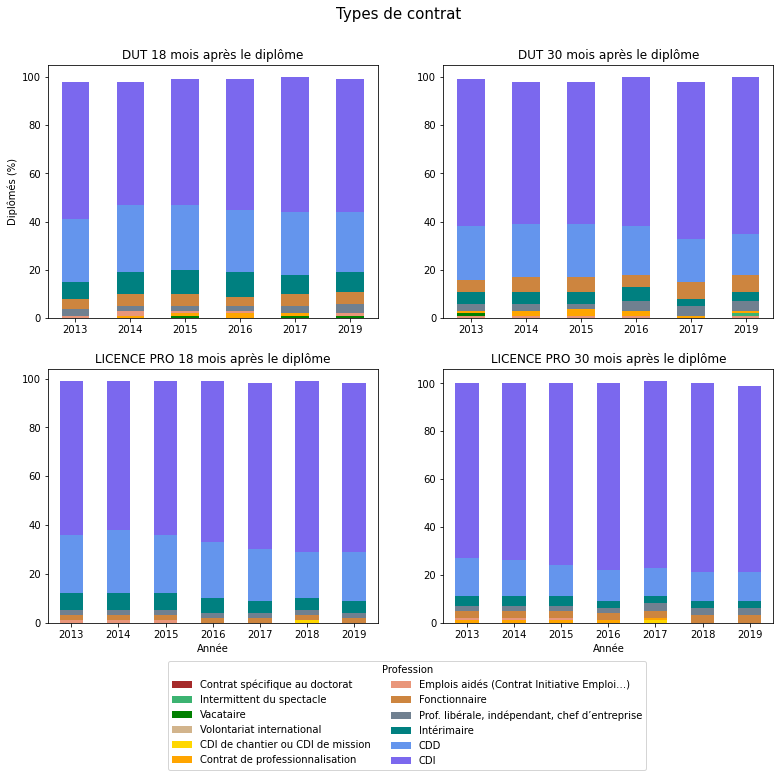
\includegraphics[width=1\textwidth]{../graphs/repartition_contrats_situation_1.png}
			\captionof{figure}{Répartition des contrats à 18 et 30 mois après l'obtention du diplôme}
			\label{fig:contrat_pourcentage_1}
		\end{figure}
	
		\begin{figure}[H]
			\centering
			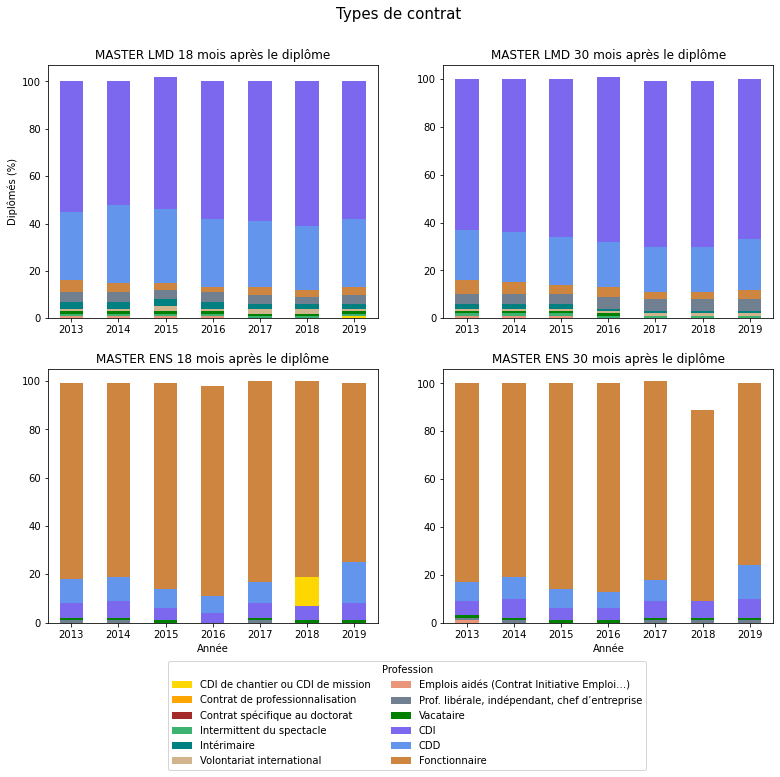
\includegraphics[width=1\textwidth]{../graphs/repartition_contrats_situation_2.png}
			\captionof{figure}{Répartition des contrats à 18 et 30 mois après l'obtention du diplôme}
			\label{fig:contrat_pourcentage_2}
		\end{figure}

\section{Les professions après l'obtention du diplôme}

	\subsection{Répartition des professions à 18 et 30 mois après l'obtention du diplôme}
		\begin{figure}[H]
			\centering
			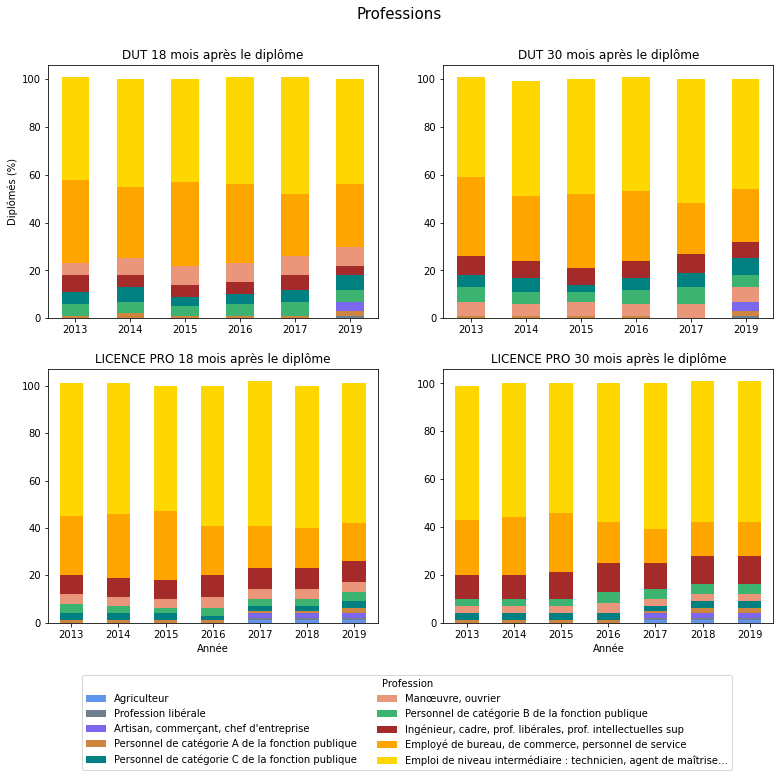
\includegraphics[width=1\textwidth]{../graphs/repartition_professions_situation_1.png}
			\captionof{figure}{Répartition des professions à 18 et 30 mois après l'obtention du diplôme (DUT-Licence pro)}
			\label{fig:profession_pourcentage_1}
		\end{figure}
	
		\begin{figure}[H]
			\centering
			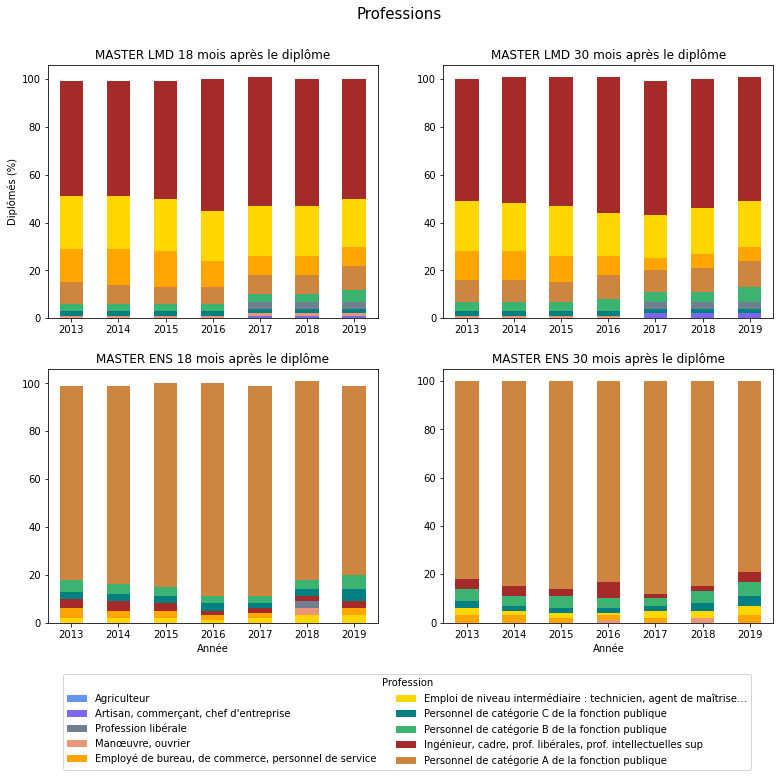
\includegraphics[width=1\textwidth]{../graphs/repartition_professions_situation_2.png}
			\captionof{figure}{Répartition des professions à 18 et 30 mois après l'obtention du diplôme (Masters)}
			\label{fig:profession_pourcentage_2}
		\end{figure}


\section{Secteurs d'activité après l'obtention du diplôme}
	Les données 18 mois après l'obtention du diplôme étant manquantes, nous indiquons dans la Figure 5, le pourcentage des secteurs d'activité dans lesquels les diplômés se sont insérés 30 mois après son obtention. 

	\begin{figure}[H]
		\centering
		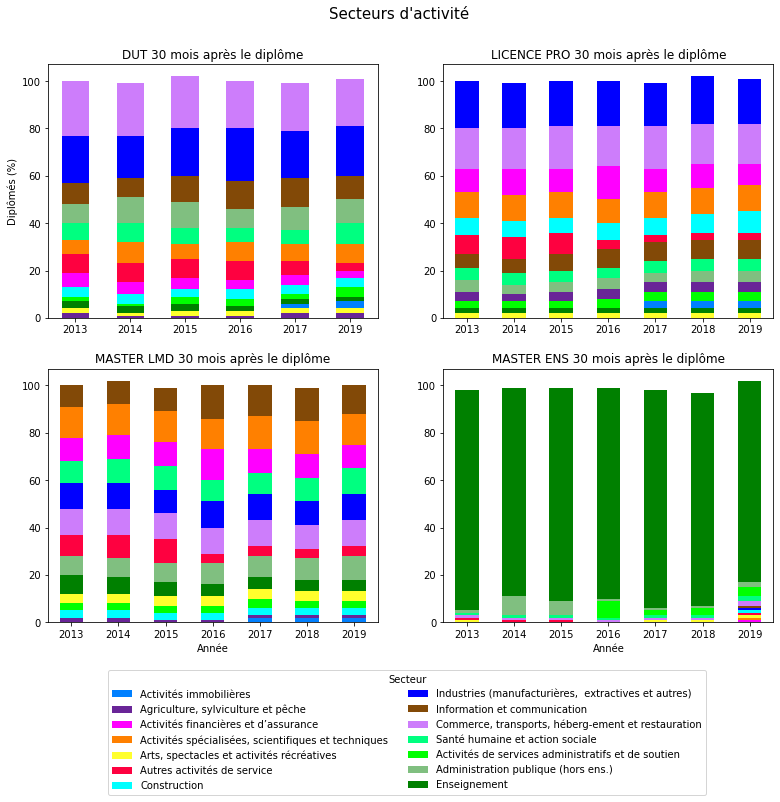
\includegraphics[width=1\textwidth]{../graphs/repartition_secteurs_situation.png}
		\captionof{figure}{Répartition des secteurs à 18 et 30 mois après l'obtention du diplôme}
	\end{figure}

\section{Proportion des diplômés et des diplômes universitaires}

	\subsection{Proportion des diplômés}
	Le Tableau \ref{tab:genre_responses} et la Figure \ref{fig:genre_reponses} fournissent la proportion des hommes et des femmes de l'ensemble des diplômés de 2013 à 2019 ayant répondu à l'enquête. Ainsi nous avons environ 22 \% de réponses à l'enquête en plus de la part des femmes par rapport au hommes, pourtant à un total d'environ 592740 de diplômés interrogés
	
		\begin{table}[H]
			\centering
			\begin{tabular}{lcc}
				\toprule
				\textbf{Genre} & \textbf{Nombre de réponses} & \textbf{\%} \\
				\midrule
				Femmes & 360364 & 60.8 \\
				Hommes & 232376 & 39.2 \\
				\bottomrule
			\end{tabular}
			\caption{Nombre et proportion de diplômés par genre (2013 à 2019)}
			\label{tab:genre_responses}
		\end{table}
	
		\begin{figure}[H]
			\centering
			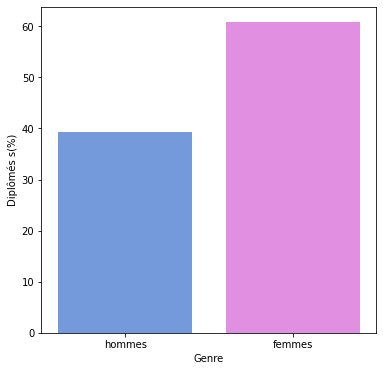
\includegraphics[width=0.6\textwidth]{../graphs/proportion_genre.png}
			\captionof{figure}{Proportion des diplômés selon le genre (2013 à 2019)}
			\label{fig:genre_reponses}
		\end{figure}
	
	\subsection{Proportion des diplômes universitaire}
	Le Tableau \ref{tab:diplome_genre} et la Figure \ref{fig:diplome_genre} présentent le nombre et la proportion de diplômés par niveau de diplôme universitaire selon le genre. 
	
		\begin{table}[H]
			\centering
			\begin{tabular}{llcc}
				\toprule
				\textbf{Diplôme} & \textbf{Genre} & \textbf{Nombre de réponses} & \textbf{\%} \\
				\midrule
				DUT & Femmes & 8560 & 1.4 \\
				& Hommes & 9328 & 1.6 \\
				\midrule
				LICENCE PRO & Femmes & 72910 & 12.3 \\
				& Hommes & 56474 & 9.5 \\
				\midrule
				MASTER ENS & Femmes & 56912 & 9.6 \\
				& Hommes & 16400 & 2.8 \\
				\midrule
				MASTER LMD & Femmes & 221982 & 37.5 \\
				& Hommes & 150174 & 25.3 \\
				\bottomrule
			\end{tabular}
			\caption{Nombre et proportion (\%) de diplômés par diplôme selon le genre (2013 à 2019)}
			\label{tab:diplome_genre}
		\end{table}
		
	Nous constatons que les diplômés de la filière des DUT sont beaucoup moins représentés (3 \%) que ceux des licences professionnelles (22 \%) et des masters LMD (75 \%). Il y a également moins de diplômés dans l'enquête pour le Master ENS avec une proportion plus forte de 6.1 \% de femmes par rapport aux hommes.
	Les Licences professionnelles et les Masters LMD rassemblent la majorité des diplômés de l'enquête avec 22 \% pour les licences pro et 63 \% pour les Masters LMD.
	Nous constatons que les femmes représentent la majorité des diplômés en Masters. Les hommes représentent environ 11 \% des diplômés en DUT et Licences professionnelles contre 14 \% pour les femmes. Mais les femmes représentent 47 \% des diplômés en Masters ayant répondu à l'enquête contre 28 \% pour les hommes.
		\begin{figure}[H]
			\centering
			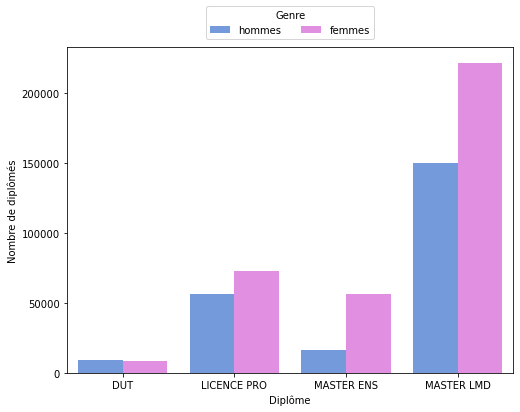
\includegraphics[width=0.8\textwidth]{../graphs/nombre_diplome_genre.png}
			\captionof{figure}{Nombre de diplômés par diplôme selon le genre (2013 à 2019)}
			\label{fig:diplome_genre}
		\end{figure}
	
	La plus forte proportion de femmes dans les filières plus longues (Masters) par rapport aux hommes est-elle liée au nombre insuffisant de réponses à l'enquête s'agissant des hommes ( -22 \% / femmes) ou bien les femmes sont-elles plus en capacité de choisir des études plus longues et moins techniques que leurs homologues masculins ?
	
	Il semblerait, dans l'hypothèse d'un effectif constant pour les femmes, que même avec 12 \% de diplômés masculins en plus, il serait difficile de rattraper les effectifs des femmes en Masters puisque le différentiel de diplômés est déjà d'environ 11 \% en faveur des femmes.      

\section{Proportion des disciplines des diplômés}

	\begin{table}[H]
		\centering
		\begin{tabular}{llcc}
			\toprule
			\textbf{Genre} & \textbf{Discipline} & \textbf{Nombre de réponses} & \textbf{\%} \\
			\midrule
			Hommes & Gestion & 29837 & 10.1 \\
			& Informatique & 16915 & 5.7 \\
			& Sciences de la vie et de la terre & 12563 & 4.2 \\
			& Sciences de l'ingénieur & 9885 & 3.3 \\
			& Lettres, langues, arts & 8326 & 2.8 \\
			& Masters enseignement & 8200 & 2.8 \\
			& Sciences fondamentales & 8169 & 2.8 \\
			& Droit & 6909 & 2.3 \\
			& Économie & 5920 & 2 \\
			& Information communication & 4879 & 1.6 \\
			& Histoire-géographie & 3590 & 1.2 \\
			& Psychologie & 1118 & 0.3 \\
			\midrule
			Femmes & Gestion & 41632 & 14 \\
			& Lettres, langues, arts & 29079 & 9.8 \\
			& Masters enseignement & 28456 & 9.6 \\
			& Sciences de la vie et de la terre & 20479 & 6.9 \\
			& Droit & 15838 & 5.3 \\
			& Information communication & 10003 & 3.4 \\
			& Sciences fondamentales & 8132 & 2.74 \\
			& Psychologie & 7949 & 2.7 \\
			& Économie & 7667 & 2.6 \\
			& Histoire-géographie & 5614 & 1.9 \\
			& Sciences de l'ingénieur & 2964 & 1 \\
			& Informatique & 2378 & 0.8 \\
			\bottomrule
		\end{tabular}
		\caption{Nombre et proportion (\%) des diplômés par discipline selon le genre (2013 à 2019)}
		\label{tab:genre_discipline}
	\end{table}

	
	Le Tableau \ref{tab:genre_discipline} et la Figure \ref{fig:genre_discipline} présentent le nombre de diplômés par discipline ainsi que leur proportion (\%) par rapport à l'ensemble des diplômés ayant répondu à l'enquête.
	Nous constatons, entre les hommes et les femmes,  une nette inversion de la proportion des disciplines  littéraires (2.8 \% contre 9.8 \%) ou dans l'enseignement (2.7 \% contre 9.6 \%) par rapport aux domaines plus techniques et scientifiques comme les sciences de l'ingénieur (3.3 \% contre 1 \%) ou encore l'informatique (5.70 \% contre 0,8 \%)

	\begin{figure}[H]
		\centering
		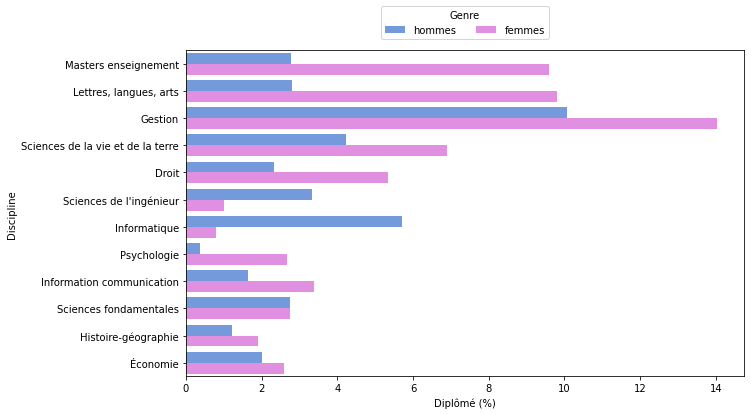
\includegraphics[width=1\textwidth]{../graphs/proportion_disciplines.png}
		\captionof{figure}{Proportion (\%) des diplômés par discipline selon le genre (2013 à 2019)}
		\label{fig:genre_discipline}
	\end{figure}

	La remarque précédente conduisant à soumettre l'hypothèse que les femmes choisiraient majoritairement les filières universitaires les plus longues (Masters) serait confirmée par les disciplines choisies.
	En effet, les domaines de l'enseignement ou encore littéraires sont des domaines dont les années d'études sont les plus longues pour aboutir à une insertion professionnelle plus prometteuse.
	Alors que les hommes à 79 \%, contre  53 \% pour les femmes,  préféraient davantage une insertion plus rapide sur le marché du travail en choisissant les sciences, davantage corrélées l'industrie ou encore en filières plus courtes, les licences professionnelles (16,8 \% contre 12,5 \%). Pourtant, la gestion reste la discipline privilégiée pour les hommes (10 \%) et les femmes (14 \%) 


\section{La question épineuse des salaires}
L’information collectée sur le salaire porte sur le salaire net, primes comprises. Dans toute la suite de l'analyse, tous les calculs statistiques sont faits à partir des salaires médians de chaque catégorie de diplôme (DUT, Licence Pro, Master LMD et ENS) et de discipline (Figure \ref{fig:genre_discipline}) et selon le genre. Il ainsi important de comprendre que les valeurs produites ici,  ne donnent qu'une indication ou une tendance et non des valeurs médianes qui aurait été plus précises avec les salaires obtenu pour chaque homme et femme interrogés.
 

	\subsection{Les quantiles des salaires}	
	Le Tableau \ref{tab:quartile_salaire_genre} et la Figure \ref{fig:boxplot_salaire_genre} montrent les différents quartiles des salaires entre les hommes et les femmes, de 18 à 30 mois après l'obtention du diplôme sur toute la période de 2013 à 2019.
	
	\begin{table}[H]
		\centering
		\begin{tabular}{lcc}
			\toprule
			\textbf{Genre} & \textbf{Quartile} & \textbf{Salaire} \\
			\midrule
			Femmes & 0.25 & 1450 \\
			& 0.50 & 1600 \\
			& 0.75 & 1800 \\
			\midrule
			Hommes & 0.25 & 1560 \\
			& 0.50 & 1730 \\
			& 0.75 & 1910 \\
			\bottomrule
		\end{tabular}
		\caption{Dispersion des salaires selon le genre (2013 à 2019)}
		\label{tab:quartile_salaire_genre}
	\end{table}
	
	
	Nous constatons, dans une première lecture, que, quelque soit la tranche des salaires, des plus faibles (1er quartile 0,25) aux plus élevés (3ème quartile), les hommes auraient tendance à percevoir des salaires supérieurs aux femmes. Nous remarquons également que l'écart, à niveau d'étude égale, reste relativement constant (environ 110 €).
		
	
	\begin{figure}[H]
		\centering
		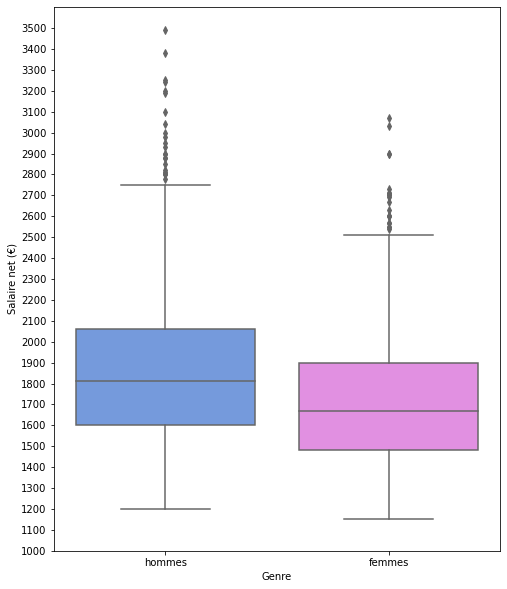
\includegraphics[width=0.7\textwidth]{../graphs/boxplot_salaire_genre.png}
		\captionof{figure}{Quartiles des salaires par genre des emplois stables (2013 à 2019)}
		\label{fig:boxplot_salaire_genre}
	\end{figure}
	

	Le Tableau \ref{tab:salaire_median_genre} et la Figure \ref{fig:salaire_median_genre} montrent le salaire net mensuel médian des emplois stables des hommes et les femmes. 
	
	\begin{table}[H]
		\centering
		\begin{tabular}{llc}
			\toprule
			\textbf{Genre} & \textbf{Diplôme} & \textbf{Salaire net mensuel médian (€)} \\
			\midrule
			Femmes & DUT & 1400 \\
			& LICENCE PRO & 1600 \\
			& MASTER ENS & 1750 \\
			& MASTER LMD & 1820 \\
			\midrule
			Hommes & DUT & 1650 \\
			& LICENCE PRO & 1730 \\
			& MASTER ENS & 1800 \\
			& MASTER LMD & 2075 \\
			\bottomrule
		\end{tabular}
		\caption{Salaire net mensuel médian des emplois à temps plein par genre et diplôme (2013 à 2019)}
		\label{tab:salaire_median_genre}
	\end{table}
	
	
	
	Nous observons que les hommes ont un salaire médian plus élevé quelques soit leur niveau de diplôme.
	Sans surprise, plus le niveau d'étude des diplômés est élevé et plus les salaires sont élevés.
	Les hommes diplômés au niveau DUT et Master auraient un salaire médian d'environ 255 € plus élevé que celui des femmes avec le même niveau d'étude.
	Nous remarquons que pour le Master enseignement (ENS) le salaire médian est pratiquement équivalent.  
	La Figure \ref{fig:contrat_pourcentage_2} nous apprend qu'au niveau des Masters ENS l'essentiel des diplômés sont dans la fonction publique après la sortie de leurs études contrairement au Masters LMD qui sont essentiellement dans le secteur privé.
		
	\begin{figure}[H]
		\centering
		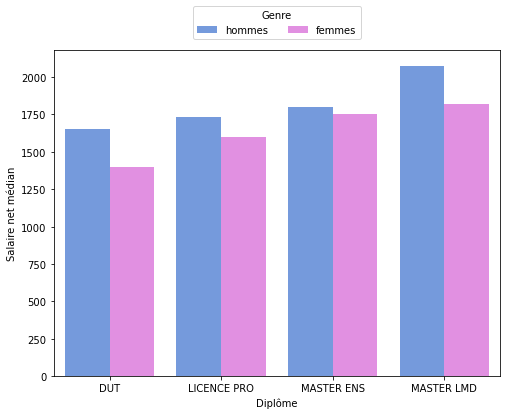
\includegraphics[width=0.7\textwidth]{../graphs/salaires_medians_genre.png}
		\captionof{figure}{Salaire net mensuel médian par genre selon le diplôme des emplois stable (2013 à 2019)}
		\label{fig:salaire_median_genre}
	\end{figure}
	Cela supposerait que les hommes choisissant majoritairement les filières scientifiques (sciences de l'ingénieur, informatique...) auraient des salaires plus élevés que les femmes avec le même niveau d'étude mais choisissant des disciplines moins rémunératrices (Gestion, lettres, enseignement, etc..).
	
	\begin{table}[H]
		\centering
		\begin{tabular}{llcr}
			\toprule
			\textbf{Genre} & \textbf{Diplôme} & \textbf{Quartile} & \textbf{Salaire} \\
			\midrule
			Femmes & DUT & 25 \% & 1290 \\
			&     & 50 \% & 1400 \\
			&     & 75 \% & 1585 \\
			\cmidrule{2-4}
			& LICENCE PRO & 25 \% & 1430 \\
			&             & 50 \% & 1585 \\
			&             & 75 \% & 1737.5 \\
			\cmidrule{2-4}
			& MASTER ENS & 25 \% & 1700 \\
			&            & 50 \% & 1750 \\
			&            & 75 \% & 1842.5 \\
			\cmidrule{2-4}
			& MASTER LMD & 25 \% & 1607.5 \\
			&            & 50 \% & 1820 \\
			&            & 75 \% & 2087.5 \\
			\midrule
			Hommes & DUT & 25 \%& 1400 \\
			&     		& 50 \% & 1600 \\
			&     & 75 \% & 1800 \\
			\cmidrule{2-4}
			& LICENCE PRO & 25 \% & 1600 \\
			&             & 50 \% & 1730 \\
			&             & 75 \% & 1950 \\
			\cmidrule{2-4}
			& MASTER ENS & 25 \% & 1700 \\
			&            & 50 \% & 1800 \\
			&            & 75 \% & 1965 \\
			\cmidrule{2-4}
			& MASTER LMD & 25 \% & 1817.5 \\
			&            & 50 \% & 2075 \\
			&            & 75 \% & 2345 \\
			\bottomrule
		\end{tabular}
		\caption{Dispersion des salaires par diplôme selon le genre (2013 à 2019)}
		\label{tab:quartile_values_diplome}
	\end{table}
	
	
	Dans le Tableau \ref{tab:quartile_values_diplome} et la Figure \ref{fig:boxplot_diplome_genre} nous observons plus en détail la répartition des quartiles selon le diplôme entre les hommes et les femmes permettant d'avoir une tendance plus précise des salaires par niveau d'étude des personnes interrogées. 
	
	Nous avons observé que les salaires augmentent selon le niveau d'étude pour les hommes et les femmes. Cependant, quelque soit le diplôme obtenu, les tranches de salaires seraient toujours plus élevés pour les hommes comparativement aux femmes à niveau d'étude équivalent.
	
	On remarque également une différence des salaires médians entre les hommes et les femmes. 
	
	Nous avons observé sur la Figure \ref{fig:contrat_pourcentage_2} et la Figure \ref{fig:profession_pourcentage_2} que les emplois des diplômés du Master ENS sont pour l'essentiel dans la fonction publique (> à 80 \%) contrairement aux autres diplômés dont les emplois sont très majoritairement dans le secteur privé ( >  à 80 \%).
	
	On pourrait donc en conclure que les écarts des salaires dans la fonction public sont moins importants que dans la fonction publique.
	
	Selon le Tableau \ref{tab:quartile_values_diplome}, il y aurait moins de 25 \% des femmes interrogées diplômées d'un Master LMD qui auraient un salaire inférieur à 1610 € et 75 \% inférieur à 2090 € avec un salaire médian de 1820 €.
	Les hommes, à niveau d'étude équivalent, auraient un salaire inférieur à 1817 € pour 25 \% d'entre eux et inférieur à 2345 € pour 75 \% d'entre eux.
	

	\begin{figure}[H]
		\centering
		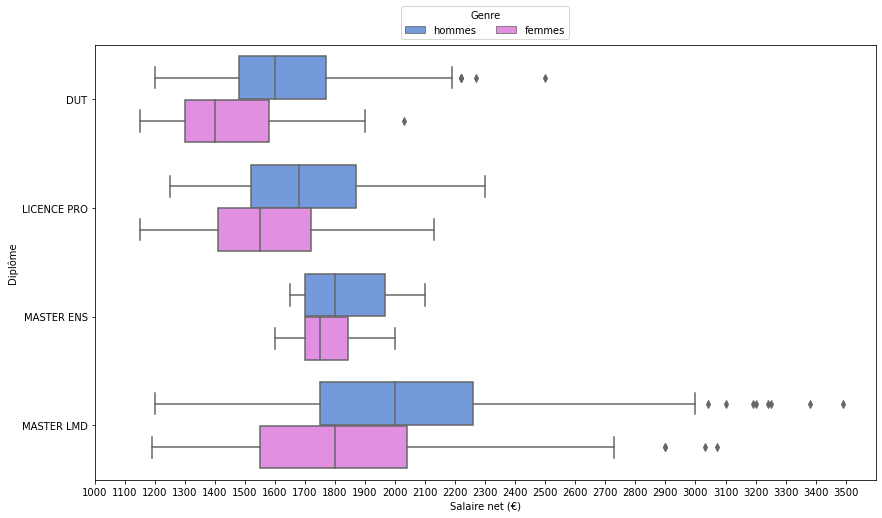
\includegraphics[width=1\textwidth]{../graphs/boxplot_diplomes_genre.png}
		\captionof{figure}{Quartiles des salaires nets mensuels des emplois stables par genre selon le diplôme (2013 à 2019)}
		\label{fig:boxplot_diplome_genre}
	\end{figure}

	Le Figure \ref{fig:boxplot_salaire_discipline} montrerait que les diplômés des disciplines en sciences de l'ingénieur, en économie, ou encore, en sciences fondamentales auraient des salaires médians supérieurs aux diplômés des autres disciplines. Le Tableau \ref{tab:diff_salaire_genre}, indique ces différences. De plus, la répartition des salaires supérieurs aux salaires médians et à peu près équivalente aux salaires qui en sont inférieurs. Cependant nous observons des écarts entre les salaires médians en faveur des hommes par rapport aux femmes.
	
	En prenant l'exemple de la gestion, la discipline où les femmes sont les plus diplômées (Figure \ref{fig:genre_discipline}, auraient environ un salaire de moins de 1300 € pour 25 \% d'entre elles et inférieur à 1750 € pour 75 \% d'entre elles.
	Alors que les hommes, dans la même discipline, auraient un salaire inférieur à 1470 € pour  25 \% d'entre eux et inférieur à 1950 € pour 75 \% d'entre eux. 
	
	Au regard de ces résultats, nous pourrions penser que les hommes sont mieux rémunérés que les femmes quelque que soit le niveau de formation et la spécialité choisie. A noter que seules les femmes diplômées en informatique auraient un salaire médian supérieur aux hommes mais cela reste modeste (< 50€). Mais c'est aussi dans ce secteur que les femmes sont les moins présentes.
	
	\begin{table}[H]
		\centering
		\begin{tabular}{lc}
			\toprule
			\textbf{Discipline} & \textbf{Différence de salaire (€)} \\
			\midrule
			Droit & 160 \\
			Gestion & 160 \\
			Histoire-géographie & 60 \\
			Information communication & 85 \\
			Informatique & -45 \\
			Lettres, langues, arts & 100 \\
			Masters enseignement & 90 \\
			Psychologie & 100 \\
			Sciences de l'ingénieur & 75 \\
			Sciences de la vie et de la terre & 45 \\
			Sciences fondamentales & 100 \\
			Économie & 190 \\
			\bottomrule
		\end{tabular}
		\caption{Différence des salaire médians des hommes par rapport aux femmes par discipline}
		\label{tab:diff_salaire_genre}
	\end{table}

	\begin{figure}[H]
		\centering
		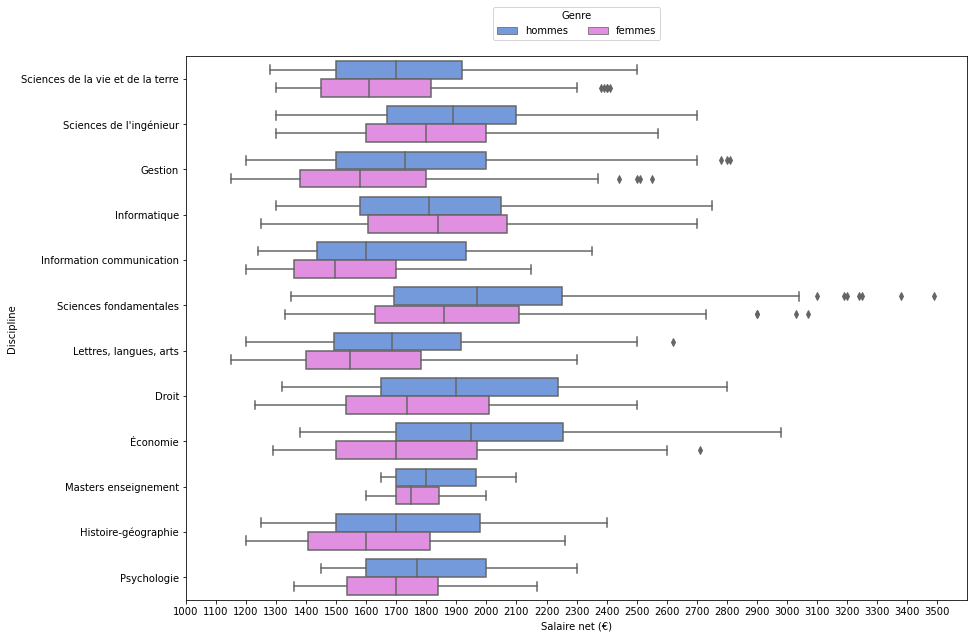
\includegraphics[width=1\textwidth]{../graphs/boxplot_salaire_discipline.png}
		\captionof{figure}{Quartiles des salaires nets mensuels des emplois stables par genre selon le diplôme (2013 à 2019)}
		\label{fig:boxplot_salaire_discipline}
	\end{figure}

\section{Taux d'insertion des diplômés dans les emplois stables}

Le taux d’insertion est défini comme étant le pourcentage de diplômés occupant un emploi, quel qu’il soit, sur l’ensemble des diplômés présents sur le marché du travail. Il est calculé sur les diplômés de nationalité française, issus de la formation initiale, entrés immédiatement et durablement sur le marché du travail après l’obtention de leur diplôme en 2013, 2014, 2015, 2016, 2017, 2018 ou 2019.
		
		\begin{figure}[H]
			\centering
			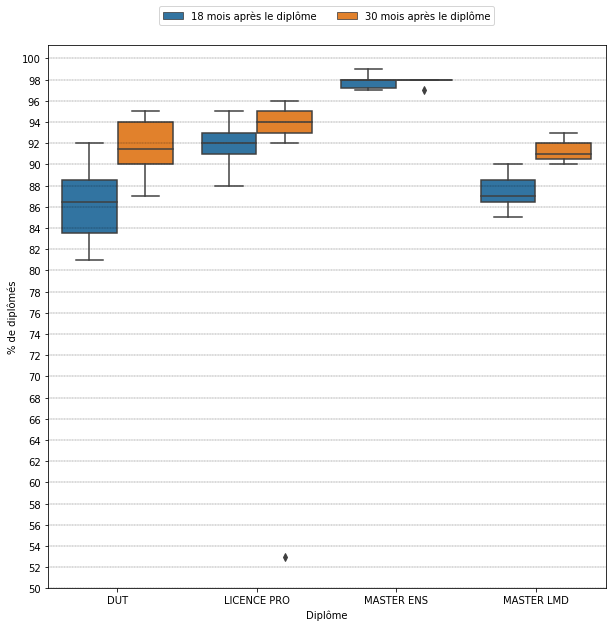
\includegraphics[width=1\textwidth]{../graphs/boxplot_insertion_diplome.png}
			\captionof{figure}{Taux d'insertion des diplômés selon leur diplôme universitaire (2013 à 2019)}
			\label{fig:boxplot_insertion_diplome}
		\end{figure}
	
	
	La Figure \ref{fig:boxplot_insertion_diplome} représente le taux d'insertion à 18 et 30 mois après l'obtention du diplôme par les interrogés de 2013 à 2019. Nous observons que les taux d'insertion sont meilleurs pour les plus diplômés.
	Les diplômés de licence professionnelle ont un taux médian d'insertion professionnelle (89 \%) supérieur aux diplômés de DUT (84 \%) ou Master LMD (88 \%). D'après la figure \ref{fig:insertion_ens} seuls les diplômés en Master ENS ont un taux d'insertion supérieur à 95 \%, proche des 98 \%.
	
	Nous remarquons que les licences professionnelles ont un taux d'insertion inférieur à 93 \% pour 75 \% d'entre eux contre 94 \% pour les DUT 30 mois après l'obtention de leur diplôme.
	
	Dans l'ensemble ce sont les diplômés de licence professionnelle qui ont un meilleur taux d'insertion professionnelle à part les diplômés de Master ENS.  
		

\end{document}